\begin{frame}{Introdução}
{Contextualização}

 \begin{figure}[htp]
	\centering
	\caption{ \centering{O enlace do mundo físico e digital}}
    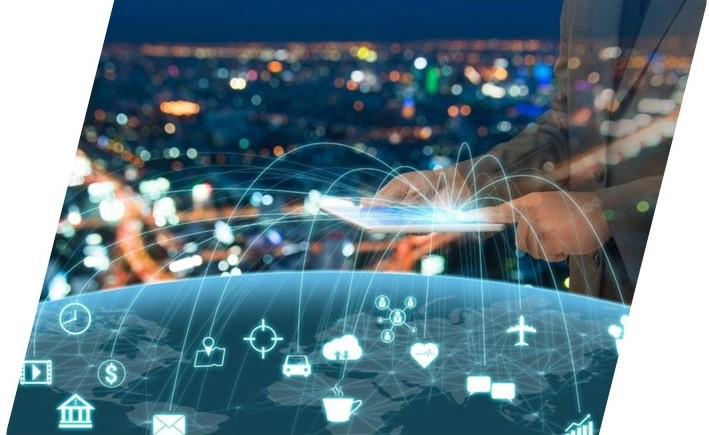
\includegraphics[width=0.5\linewidth]{img/fidi.jpg}
    \hspace{5cm}
	\legend{Fonte: Adaptado  \cite{proconcept}}
\end{figure}
 
\begin{itemize}
\item Convergências Tecnológicas: Paradigmas "\textit{Smart}";
\item Estruturas Legadas.
 \end{itemize}
\end{frame}

\begin{frame}{Introdução}{Problema de Pesquisa}
	\vspace{-0.64cm}
	\begin{figure}[htp]
		\centering
		\caption{\centering{\small{Sistema legado de iluminação e medição de energia predial}}}
		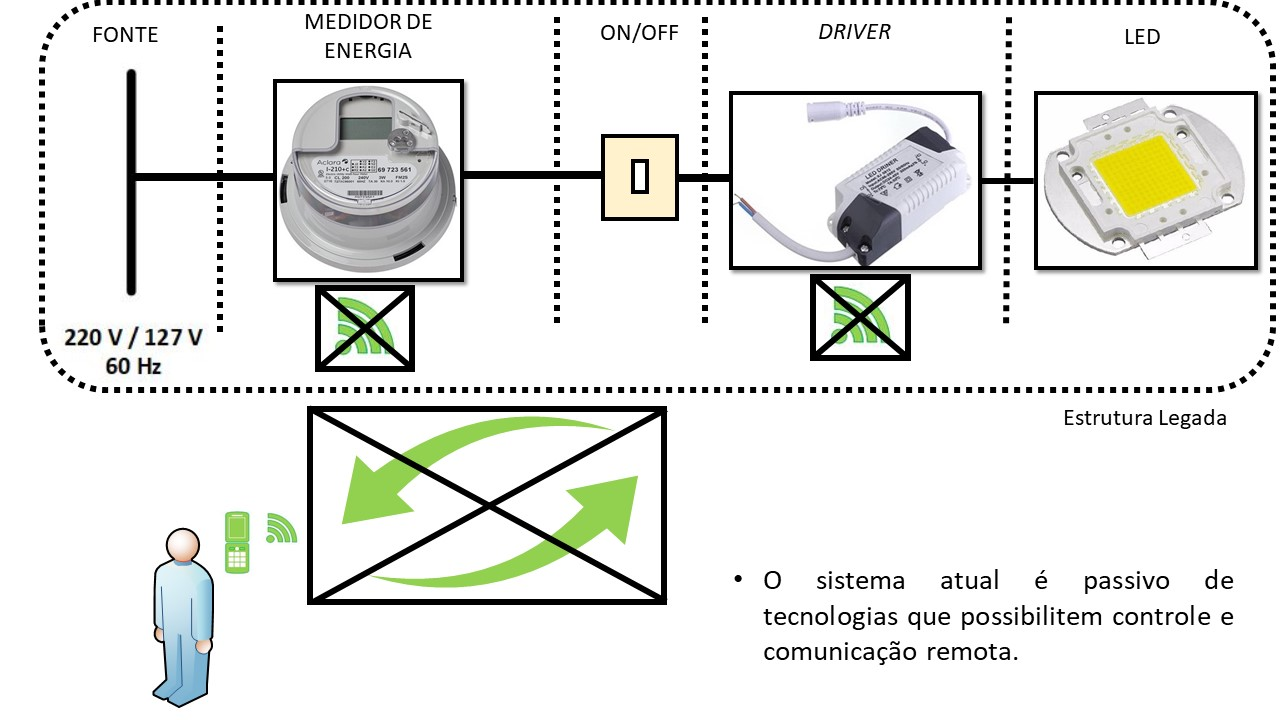
\includegraphics[width=0.97\linewidth]{img/1.jpg}
	    \hspace{5cm}
	    \vspace{5cm}
		\legend{\small{Fonte: Adaptado \cite{gomes,fernandes2018implementation,medidor}}}
	\end{figure}

\end{frame}

\begin{frame}{Introdução}{Problema de Pesquisa}
\vspace{-0.64cm}
	\begin{figure}[htp]
		\centering
		\caption{\centering{\small{Uma alternativa a convergência \textit{Smart Building}}}}
		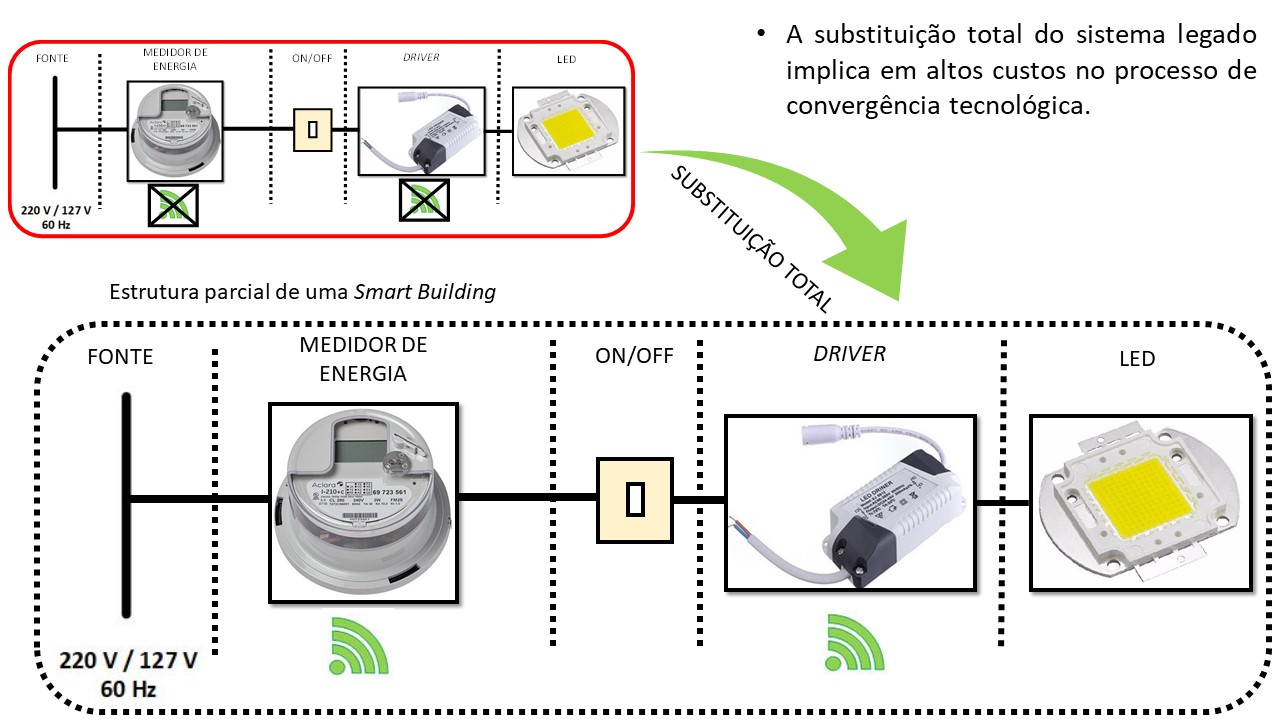
\includegraphics[width=0.97\linewidth]{img/2.jpg}
	    \hspace{5cm}
	    \vspace{5cm}
		\legend{\small{Fonte: Adaptado \cite{gomes,fernandes2018implementation,medidor}}}
	\end{figure}

\end{frame}


\begin{frame}{Introdução}{Problema de Pesquisa}
\vspace{-0.64cm}
\begin{figure}[htp]
	\centering
	\caption{\centering{\small{Como efetuar a convergência \textit{Smart Building}?}}}
	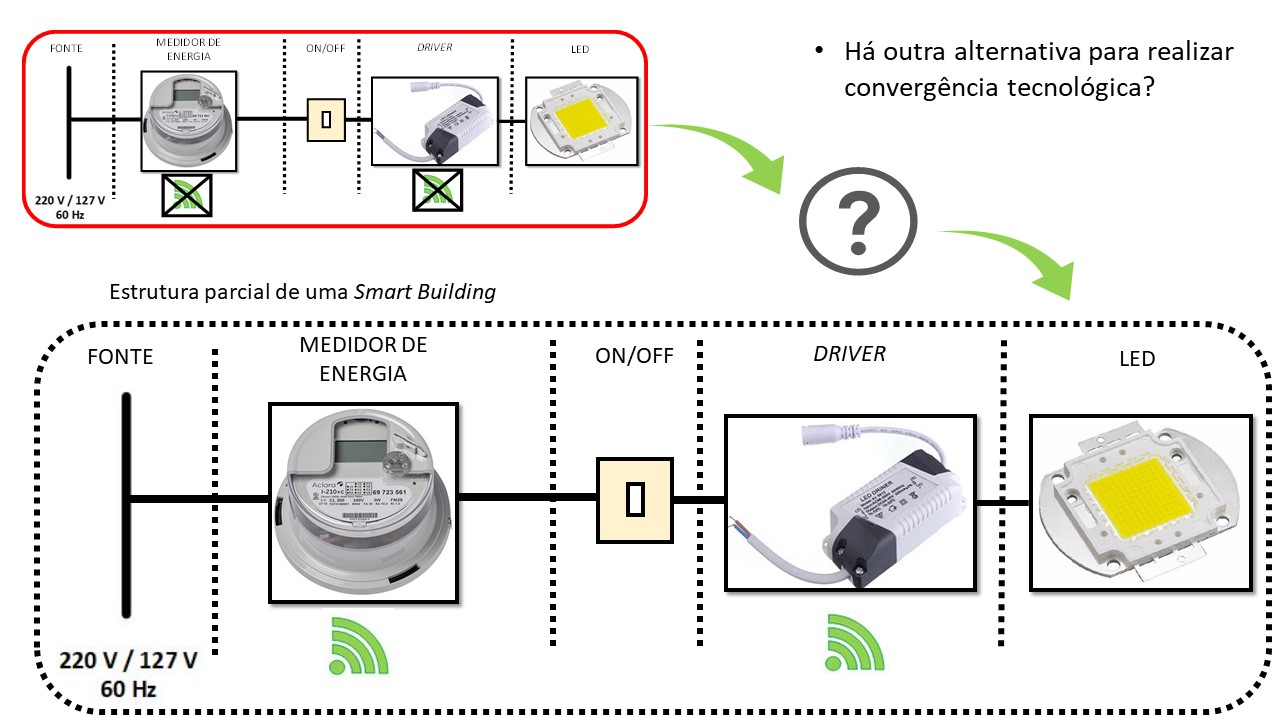
\includegraphics[width=0.97\linewidth]{img/3.jpg}
    \hspace{5cm}
    \vspace{5cm}
	\legend{\small{Fonte: Adaptado \cite{gomes,fernandes2018implementation,medidor}}}
\end{figure}

\end{frame}


\begin{frame}{Introdução}{Hipótese}
\vspace{-0.64cm}
\begin{figure}[htp]
	\centering
	\caption{\centering{\small{A estratégia do \textit{retrofit}}}}
	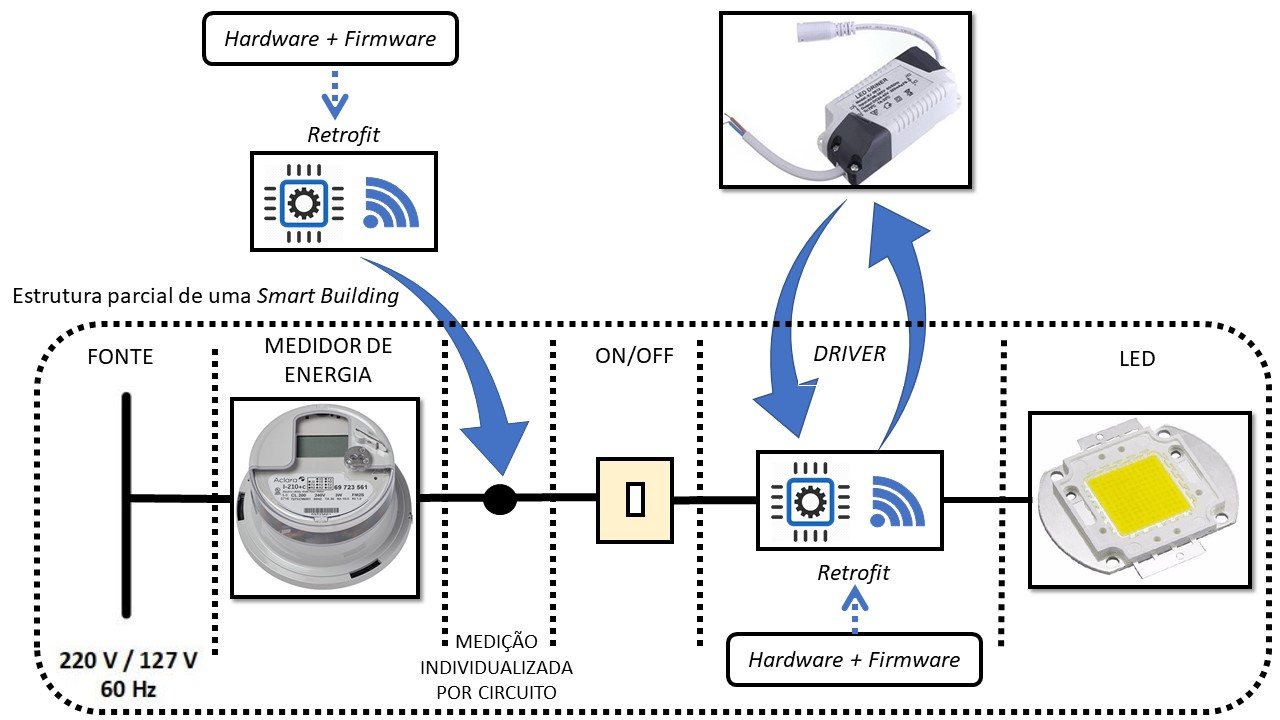
\includegraphics[width=0.97\linewidth]{img/4.jpg}
    \hspace{5cm}
    \vspace{5cm}
	\legend{\small{Fonte: Adaptado \cite{gomes,fernandes2018implementation,medidor}}}
\end{figure}

\end{frame}


\begin{frame}{Introdução}{Hipótese}
\vspace{-0.64cm}
\begin{figure}[htp]
	\centering
	\caption{\centering{\small{O \textit{retrofit} associado a plataforma SmartLVGrid para realizar a convergência \textit{Smart Building}}}}
	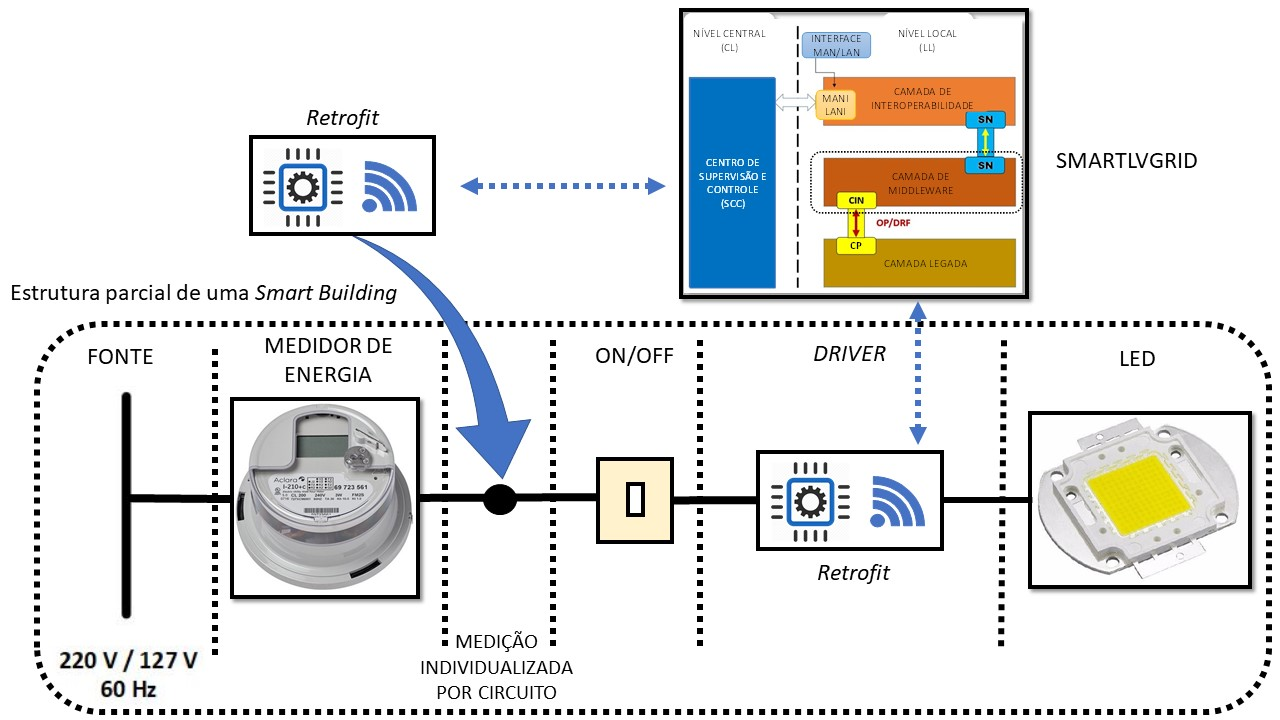
\includegraphics[width=0.915\linewidth]{img/5.jpg}
    \hspace{5cm}
    \vspace{5cm}
	\legend{\small{Fonte: Adaptado \cite{gomes,fernandes2018implementation,medidor}}}
\end{figure}

\end{frame}

\begin{frame}{Introdução}{Justificativas}
\vspace{-0.64cm}
\begin{figure}[htp]
	\centering
	\caption{\centering{\small{Justificativas do projeto}}}
	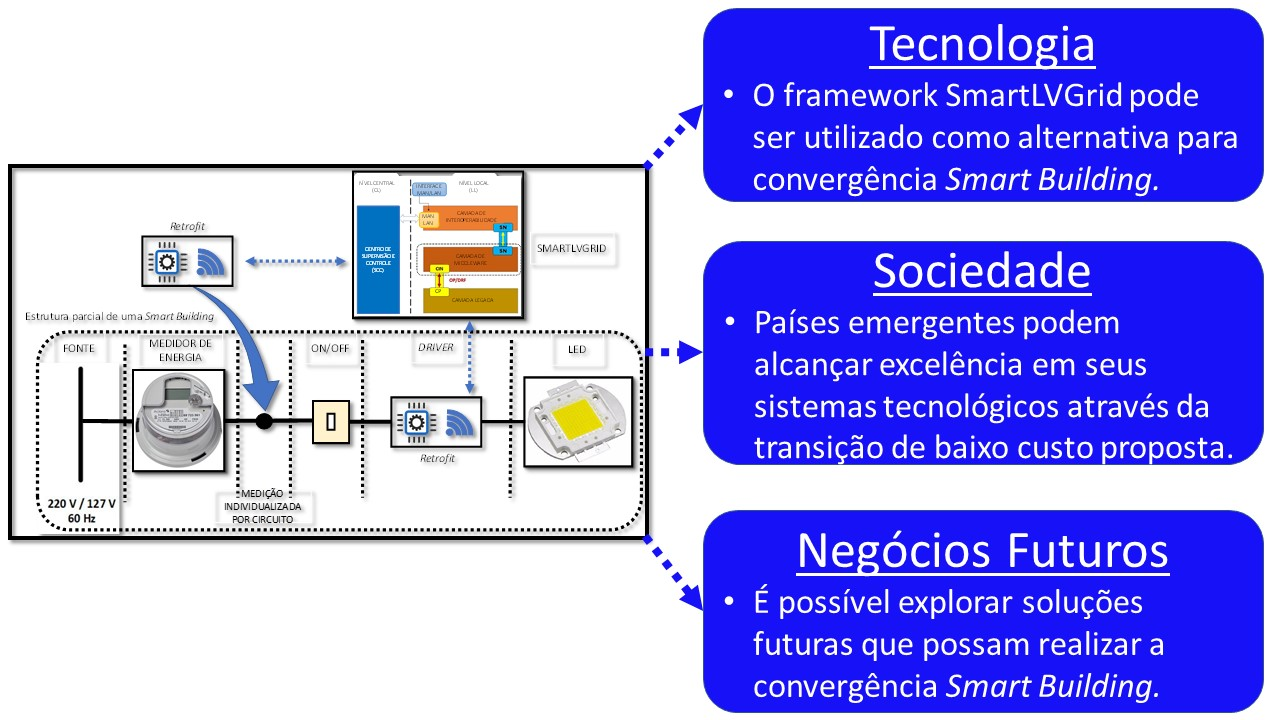
\includegraphics[width=0.97\linewidth]{img/6.jpg}
    \hspace{5cm}
    \vspace{5cm}
	\legend{\small{Fonte: Adaptado \cite{gomes,fernandes2018implementation,medidor}}}
\end{figure}

\end{frame}

\begin{frame}{Introdução}{Objetivos}
\begin{block}{Objetivo Geral}
\justify{\small{Desenvolver plataformas de \textit{hardware} e\textit{ firmware}, a camada de
\textit{middleware} do \textit{framework} SmartLVGrid, aplicadas ao retrofit de luminárias LED e de circuitos
de medição de energia elétrica, de forma a viabilizar a convergência \textit{smart building} de circuitos elétricos e iluminação de ambientes e melhorar a eficiência energética.}}
\end{block}

\begin{block}{Objetivos Específicos}
\begin{itemize}
\small{	\item definir contornos conceituais do \textit{framework} SmartLVGrid e do paradigma \textit{smart building};
	\item estudar soluções para controle de sistemas de iluminação LED e para telemedição de parâmetros elétricos;
	\item projetar e implementar módulos embarcados de \textit{retrofit} de acordo com o \textit{framework} SmartLVGrid;
	\item realizar análises dos resultados obtidos no processo de convergência \textit{smart building} com o uso do SmartLVGrid.}
\end{itemize}
\end{block}
\end{frame}

